\documentclass[a4paper,10pt]{article}
\setlength{\parindent}{0ex}
\setlength{\parskip}{1.5ex}
\usepackage[dvips]{graphicx}
\usepackage {epsfig}
\usepackage[a4paper, hmargin=25mm, vmargin=20mm, nohead]{geometry}

%INCLUDE OUR GLOBALS
\usepackage{rex201}
\usepackage{styles201}
\usepackage{ex201}


\begin{document}
\EXTESTHEADING{\INTERNO}{\INTERTESTDATE}

%{\centering \large \bf THE UNIVERSITY OF WAIKATO\\}
%{\centering \large \bf Department of Computer Science\\[0.5cm]}

%{\centering \large \bf 0657.201 Computer Systems 2002\\}
%{\centering \large \bf Exercise 7 Test - 30th July 2002\\[1cm]}

%\hrule

\begin{enumerate}
\item True/False answers. Indicate on your answer sheet if the
following statements are true or false.

\begin{enumerate}

\item When setting up exceptions, the address of your exception
handler should be loaded into the Exception Address Register
(\reg{ear})

\item Software exceptions can be disabled on the WRAMP processor.

\item Interrupts are disabled when an exception occurs.

\item When an exception occurs the cause can be determined by
examining the Exception Status Register (\reg{estat})

\item If an interrupt is not acknowledged then it will not occur again
until it is acknowledged.

\end{enumerate}

\marks{5}

\item State two main effects the \src{'rfe'} instruction has when
executed. In particular state any special registers that this
instruction changes, or uses.

\marks{3}

\item Examine the code provided in Figure~\ref{code:timer} that sets
up the Timer. Using the specifications of the REX Timer device
provided in Appendix~\ref{appen:timer}, determine the delay between
timer interrupts (in seconds).

\marks{2}
\begin{figure}[h]
\begin{small}
\begin{center}
\begin{tabular}{|p{6cm}|}
\hline
\begin{verbatim}
  1:   sw    $0, 0x72003($0)
  2:   addi  $1, $0, 12000
  3:   sw    $1, 0x72001($0)
  4:   addi  $1, $0, 0x3
  5:   sw    $1, 0x72000($0)
\end{verbatim}
\\ \hline
\end{tabular}
\end{center}
\end{small}
\caption{Timer Setup Code}
\label{code:timer}
\end{figure}

\item Provided in Figure~\ref{code:badack} is some code which should
use the REX board timer to provide an interrupt once per second. Each
time an interrupt occurs an \src{'X'} should be printed. When the code is
executed however, the program pauses for one second, and then
continuously displays \src{X}'s on the Terminal.

\label{ques:badack}

\begin{enumerate}
\item What is the error in the code that causes this problem ?
\marks{1}

\item Explain why this error results in the above behaviour.
\marks{2}

\item State the changes that you would make to ensure the code worked
as it should. You should provide the line numbers of any code that you
would change or the location that you would insert any new code into.
\marks{2}

\end{enumerate}

\begin{figure}[p]
\begin{footnotesize}
\begin{center}
\begin{tabular}{|p{12cm}|}
\hline
\begin{verbatim}
   1:  .text
   2:  .global main
   3:  main:
   4:    # Get the old exception vector
   5:    movsg  $2, $evec
   6:    # ...and save it.
   7:    sw     $2, old_vector($0)
   8:    # Get the address of my exception handler
   9:    la     $2, handler
  10:    # put it into the exception vector register
  11:    movgs  $evec, $2
  12:
  13:    # Get the CPU control register
  14:    movsg  $2, $cctrl
  15:    # Mask out all interrupts
  16:    andi   $2, $2, 0xf
  17:    # Enable IRQ2 (Timer) and Interrupt Enable.
  18:    ori    $2, $2, 0x42
  19:    # Replace the CPU control register
  20:    movgs  $cctrl, $2
  21:    
  22:    # Acknowledge any outstanding timer interrupts
  23:    sw     $0, 0x72003($0)
  24:    # Setup the delay between interrupts to 1 second.
  25:    addi   $2, $0, 2400
  26:    sw     $2, 0x72001($0)
  27:    # Setup the timer control register (AutoRestart and Timer Enable)
  28:    addi   $2, $0, 0x3
  29:    sw     $2, 0x72000($0)
  30:    
  31:  loop:   # Begin our main loop
  32:    # Read from the switches
  33:    lw     $2, 0x73000($0)
  34:    # Display the value on the SSDs
  35:    sw     $2, 0x73003($0)
  36:    srli   $2, $2, 4
  37:    sw     $2, 0x73002($0)
  38:    j      loop
  39:    
  40:  handler:
  41:    # Check the cause of the exception
  42:    movsg  $1, $estat
  43:    andi   $1, $1, 0xffb0
  44:    
  45:    # If timer then go to handle_interrupt
  46:    beqz   $1, handle_interrupt
  47:    
  48:    # Otherwise go to the system exception handler
  49:    lw     $1, old_vector($0)
  50:    jr     $1
  51:    
  52:  handle_interrupt:
  53:    # Check the serial status register
  54:    lw     $1, 0x71003($0)
  55:    # Check the transmit data sent bit
  56:    andi   $1, $1, 0x2
  57:    # Wait for the previous character to be sent
  58:    beqz   $1, handle_interrupt
  59:    # Send an 'X' to the terminal
  60:    addi   $1, $0, 'X'
  61:    sw     $1, 0x71000($0)
  62:    
  63:    # Return to the mainline
  64:    rfe
  65:
  66:  .data
  67:  old_vector:
  68:    .word  0
\end{verbatim}
\\ \hline
\end{tabular}
\end{center}
\end{footnotesize}
\caption{Code for Question~\ref{ques:badack}}
\label{code:badack}
\end{figure}

\item Figure~\ref{code:handler} shows the code for the start of an
exception handler. This code is designed to distinguish between the
different sources of exceptions and decide which, of two handlers to
run.

The address of the previous exception handler routine was saved to the
memory location specified by the label \src{'old\_vector'} during
the initialisation phase of the program.

The provided code will transfer control either to the
\src{'my\_handler'} routine, or to the system exception handler
routine as specified by the address stored in the
\src{'old\_vector'} location.

For each of the possible exception sources given in
Table~\ref{table:esources} state which routine this code will transfer
control to if that exception had occurred. You should include all
working. The format of the \reg{estat} register is provided in
Appendix~\ref{appen:estat}

\marks{5}

\begin{table}[h]
\begin{center}
\begin{tabular}{|l|l|}
\hline
IRQ0 & IRQ4, Serial Port 1 Interrupt \\
\hline
IRQ1, User Interrupt Button & IRQ5, Serial Port 2 Interrupt\\
\hline
IRQ2, Timer Interrupt & IRQ6 \\
\hline
IRQ3, Parallel Interrupt & IRQ7 \\
\hline
Arithmetic Exception & Breakpoint Exception \\
\hline
System Call Exception & General Protection Fault Exception \\
\hline
\end{tabular}
\end{center}
\caption{Exception sources for the WRAMP processor}
\label{table:esources}
\end{table}

\begin{figure}[h]
\begin{small}
\begin{center}
\begin{tabular}{|p{9cm}|}
\hline
\begin{verbatim}
   1:  handler:
   2:    # Get the exception status register
   3:    movsg  $1, $estat
   4:
   5:    andi   $1, $1, 0x7cb0
   6:
   7:    # If zero transfer control to my_handler
   8:    beqz   $1, my_handler
   9:
  10:    # Otherwise go to the system handler
  11:    lw     $1, old_vector($0)
  12:    jr     $1
  13:
  14:  my_handler:
  15:      . . . 	
\end{verbatim}
\\ \hline
% Will handle Arithmetic Exceptions, IRQ4, IRQ5, and IRQ2
\end{tabular}
\end{center}
\end{small}
\caption{Start of Exception Handler}
\label{code:handler}
\end{figure}
\end{enumerate}

\newpage
\appendix
\section{Programmable Timer}
\label{appen:timer}

The Programmable Timer on the REX board provides for generation of
interrupts at time intervals from about 1ms to 30s, with a resolution
of around 0.5ms.

The timer has an internal 16 bit register. This register is
decremented at a constant rate of 2400Hz. Once this register reaches
\src{0x0000} an interrupt is triggered. The starting value for the
timer is controlled by altering the value in the timer load register.

The timer can be configured to automatically reload the starting count
value and continue counting immediately after it expires.

The programmers view of the timer consists of four registers.  The
names of these registers and their addresses, expressed as offsets
from the base address, are provided in
Table~\ref{table:timer_offsets}.  The base address for the timer is
\src{\LOCTIMEBASE}.

\begin{table}[h]
\begin{center}
\begin{tabular}{|l|c|}
\hline
\textbf{Register name} & \textbf{Offset} \\
\hline
Timer Control Register & 0 \\
\hline
Timer Load Register & 1 \\
\hline
Timer Count Register & 2 \\
\hline
Timer Interrupt Acknowledge Register & 3 \\
\hline
\end{tabular}
\caption{Timer Register Offsets}
\label{table:timer_offsets}
\end{center}
\end{table}


\subsection{Timer Control Register}

The Timer Control Register is a read/write register, that allows the
user to enable and control aspects of the timer operation. The timer
has two primary modes of operation, automatic restart and single-shot
mode. If the timer is set to automatic restart, as soon as the timer
expires, an interrupt is triggered and the timer immediately starts
counting down again. In single-shot mode the timer will copy the value
from the timer load register only once when the timer is enabled and
will count down to zero. Once the timer reaches zero an interrupt will
be triggered and the timer will be disabled.

\begin{figure}[h]
\begin{center}
\includegraphics[width=0.8\textwidth]{timer_cr.eps}
\caption{The Timer Control Register}
\label{timer_cr_pic}
\end{center}
\end{figure}

\subsection{Timer Load Register}

The Timer Load Register is a read/write register. This register allows
the user to specify the starting count value. The starting count value
is a 16 bit value with the upper 16 bits being ignored.

\subsection{Timer Count Register}

The Timer Count Register is a read-only register. Reading from this
register returns the current value in the 16 bit internal count
register.

\subsection{Timer Interrupt Acknowledge Register}

The Interrupt Acknowledge Register is a read/write register. This
register allows a program to detect a timer overrun as as well as
acknowledge interrupts that have been dealt with.

The overrun detected bit will be set if the timer is set to automatic
restart and the timer expired again before the previous interrupt was
acknowledged. This allows a program to detect if it is unable to
service the timer interrupt fast enough.

The overrun bit must be manually reset by writing a `\src{0}' to
it's location.

\begin{figure}[h]
\begin{center}
\includegraphics[width=0.8\textwidth]{timer_iack.eps}
\caption{The Timer Interrupt Acknowledge Register}
\label{timer_iack_pic}
\end{center}
\end{figure}

eg. If the value `\src{11}' was read from the interrupt acknowledge
register we could determine that the timer has overrun since we last
acknowledged an interrupt. If `\src{00}' was written to the timer
interrupt acknowledge register we will acknowledge any outstanding
interrupts and ensure the overrun bit is reset to zero.

\subsection{Timer Example}

To configure the timer to interrupt at a specific period the first
step is to calculate the timer load value. This value can be
calculated simply by multiplying the timer frequency by the required
time between interrupts. For example, if we want the timer to generate
an interrupt once every ten seconds we would calculate it as follows:

\begin{center}
Timer Load = 2400Hz * 10s = 24000
\end{center}

Some simple code to initialise the timer to automatically restart and
to interrupt once every ten seconds is given in
Figure~\ref{code:timer_init}.

\begin{figure}[h]
\begin{footnotesize}
\begin{center}
\begin{tabular}{|p{8cm}|}
\hline
\begin{verbatim}
            . . .
           # Make sure there are no old interrupts
           # still hanging around
           sw   $0, 0x72003($0)
           # Put our auto load value in
           addi $11, $0, 24000
           sw   $11, 0x72001($0)
           # Enable the timer and autorestart
           addi $11, $0, 0x3
           sw   $11, 0x72000($0)
            . . .
\end{verbatim}
\\
\hline
\end{tabular}
\end{center}
\end{footnotesize}
\caption{Simple Timer Initialisation}
\label{code:timer_init}
\end{figure}

\newpage
\section{\$estat - Exception Status Register}
\label{appen:estat}

\begin{figure}[h]
\begin{center}
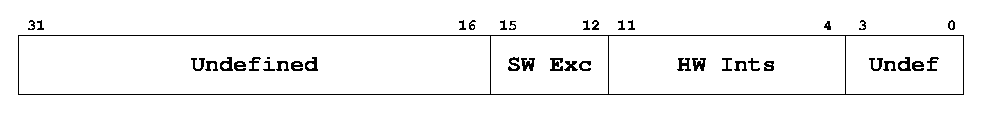
\includegraphics[width=\textwidth]{estat.eps}
\caption{\$estat - Exception Status Register}
\label{estat_pic}
\end{center}
\end{figure}

The exception status register provides the exception handler with the
ability to discover what exceptions caused it to be called. The
exception status register has a single bit flag for each external IRQ
line. Bit 4 of the status register corresponds to IRQ0, bit 5 to IRQ 1
and so on. In addition to the eight external interrupt sources the
status register also provides the status for the four CPU internal
exception sources.

The full list of all exception sources and their related status
register bit is given in Table~\ref{table:sta_loc}.

\begin{table}[h]
\begin{center}
\begin{tabular}{|l|c|}
\hline
\textbf{Exception source} & \textbf{Bit location} \\
\hline
IRQ0 & 4 \\
\hline
IRQ1 - User Interrupt Button & 5 \\
\hline
IRQ2 - Timer Interrupt & 6 \\
\hline
IRQ3 - Parallel Interrupt & 7 \\
\hline
IRQ4 - Serial Port 1 Interrupt & 8 \\
\hline
IRQ5 - Serial Port 2 Interrupt & 9 \\
\hline
IRQ6 & 10 \\
\hline
IRQ7 & 11 \\
\hline
General Protection Fault Exception & 12 \\
\hline
System Call Exception & 13 \\
\hline
Breakpoint Exception & 14 \\
\hline
Arithmetic Exception & 15 \\
\hline
\end{tabular}
\caption{Exception Status Register Fields}
\label{table:sta_loc}
\end{center}
\end{table}

\end{document}




